\chapter{L'œil et ses photorécepteurs}\label{ch:g11:the-eye}

Par une nuit sans lune, loin de toute lampe, vous voyez le chemin mais
non ses couleurs~; la veste rouge d'un ami n'est qu'une forme grise.
Regardez droit une étoile faible et elle disparaît~; regardez un peu à
côté et elle revient. Ces deux bizarreries viennent de la rétine, la
fine nappe au fond de l'\omterm{def:g11:the-eye:parts}{œil} où la lumière devient signal nerveux~: deux
sortes de \omterm{def:g10:cells-common-unit:cell}{cellules} réceptrices, inégalement réparties, l'une aveugle
aux couleurs et l'autre aveugle dans le noir. Ce chapitre démonte
l'\omterm{def:g11:the-eye:parts}{œil}, de la cornée au nerf optique, et lit, dans les \omterm{def:g10:universal-dna:gene}{gènes} des
pigments de la rétine, un morceau de notre histoire évolutive.

\section{L'œil comme instrument d'optique}

\begin{definition}[Les parties de l'œil]\label{def:g11:the-eye:parts}
L'\emph{œil}\index{œil} est un globe d'environ \qty{24}{mm} de
diamètre. La lumière entre par la \emph{cornée} transparente, franchit
la \emph{pupille} --- l'ouverture de l'\emph{iris} coloré, qui
s'élargit dans l'obscurité et se resserre en pleine lumière --- puis le
\emph{cristallin}, traverse la gelée claire du \emph{corps vitré} et
atteint la \emph{rétine}, la couche sensible à la lumière qui tapisse
le fond du globe. La cornée et le cristallin forment ensemble, sur la
rétine, une petite image renversée de la scène~; le cristallin, dont
des muscles peuvent changer la courbure, règle la mise au point du
lointain au proche (l'\emph{accommodation}). Le \emph{nerf optique}
quitte le fond de l'œil en portant au cerveau les signaux de la rétine.
\end{definition}

\begin{omfigure}
\begin{tikzpicture}
  \node[anchor=south west, inner sep=0] (img) at (0,0)
    {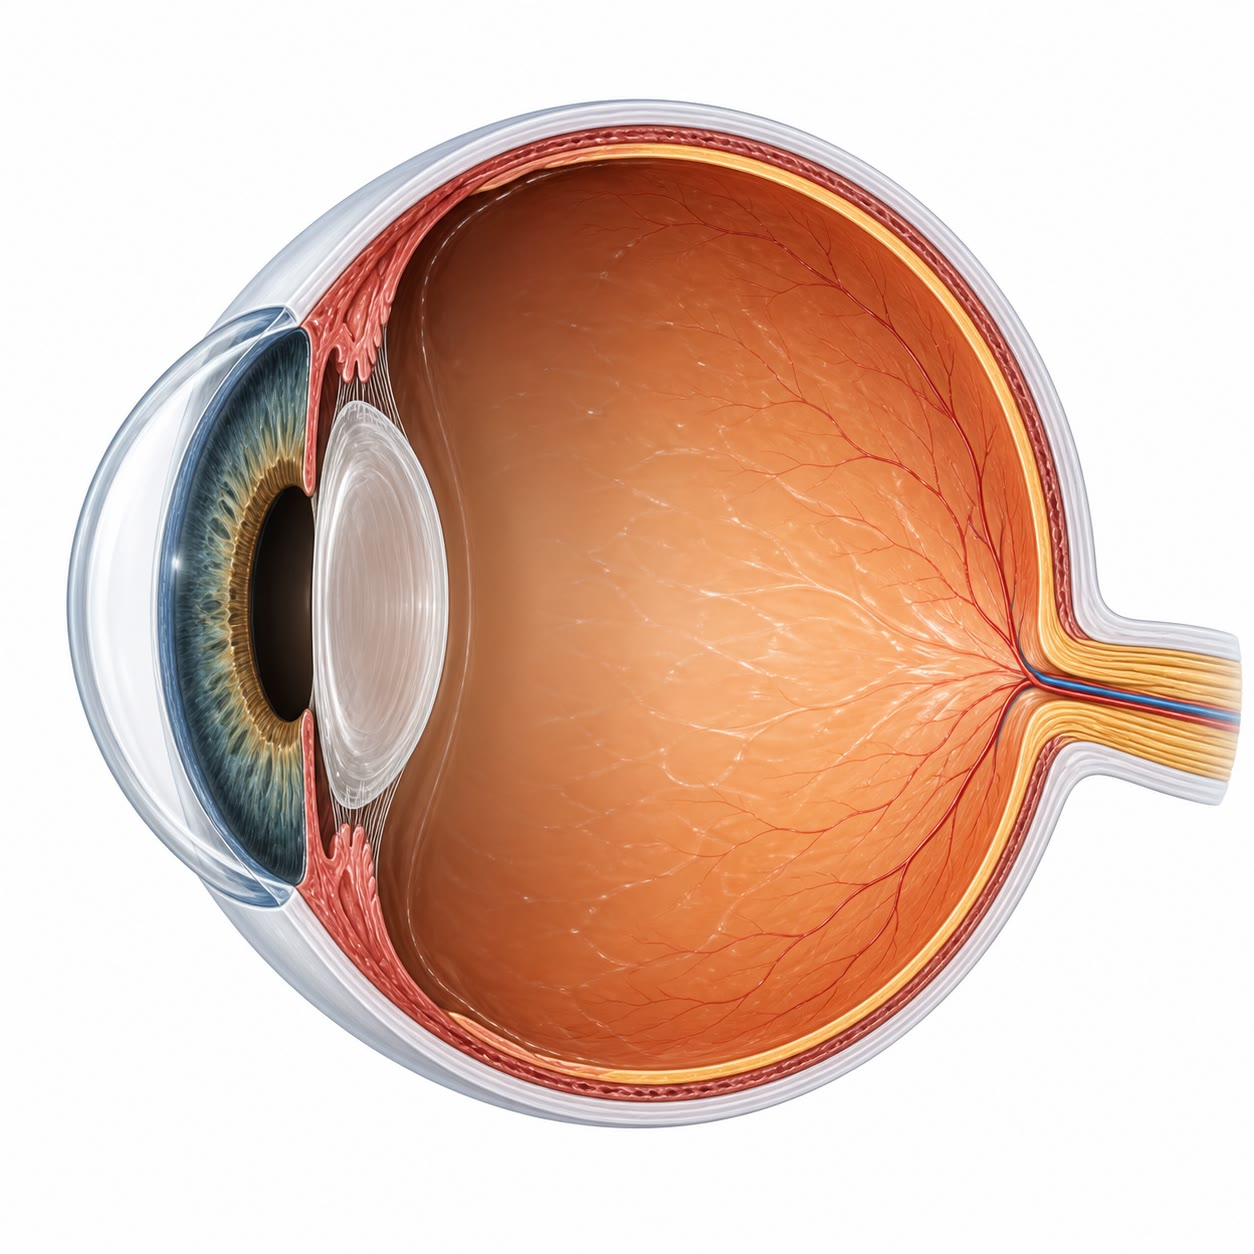
\includegraphics[width=0.46\linewidth]{images/book2/ai/fig-eye-cutaway.jpg}};
  \begin{scope}[x={(img.south east)}, y={(img.north west)},
      every node/.style={font=\small}]
    \draw[omDef, thick] (0.10,0.55) -- (-0.05,0.80) node[left] {cornée};
    \draw[omDef, thick] (0.18,0.36) -- (-0.05,0.20) node[left] {iris et pupille};
    \draw[omDef, thick] (0.26,0.50) -- (-0.05,0.50) node[left] {cristallin};
    \draw[omDef, thick] (0.55,0.50) -- (0.55,-0.06) node[below] {corps vitré};
    \draw[omDef, thick] (0.83,0.76) -- (1.05,0.88) node[right] {rétine};
    \draw[omDef, thick] (0.95,0.40) -- (1.05,0.20) node[right] {nerf optique};
  \end{scope}
\end{tikzpicture}

{\small L'\omterm{def:g11:the-eye:parts}{œil} en coupe horizontale. La cornée et le cristallin
concentrent la lumière~; la rétine, au fond, la convertit en signaux qui
partent par le nerf optique.}
\end{omfigure}

\begin{example}[La mise au point, et ses défauts]\label{ex:g11:the-eye:focus}
Un \omterm{def:g11:the-eye:parts}{œil} au repos met au point sur la rétine les objets lointains~; pour
lire à \qty{25}{cm}, le cristallin doit se bomber. Un \omterm{def:g11:the-eye:parts}{œil} un peu trop
long met au point les objets lointains en avant de la rétine --- c'est
la myopie, corrigée par un verre divergent~; un \omterm{def:g11:the-eye:parts}{œil} trop court, ou un
cristallin durci par l'âge, ne parvient pas à mettre au point les
objets proches --- c'est l'hypermétropie, corrigée par un verre
convergent. Dans chaque cas, la rétine est intacte~: le défaut est
optique, et les lunettes replacent l'image là où sont les récepteurs.
\end{example}

\section{La rétine}

\begin{definition}[Photorécepteurs]\label{def:g11:the-eye:photoreceptors}
La rétine contient deux sortes de \omterm{def:g10:cells-common-unit:cell}{cellules}
\emph{photoréceptrices}\index{photorécepteur}, nommées d'après leur
forme. Les \emph{bâtonnets}\index{bâtonnet (rétine)}, environ 120
millions, répondent à une lumière très faible mais tous avec le même
pigment~: ils donnent une vision en nuances de gris la nuit. Les
\emph{cônes}\index{cône (rétine)}, environ 6 millions, exigent une
lumière plus vive et se déclinent en trois types, chacun avec un
pigment le plus sensible à une région différente du spectre~: ils
donnent la vision diurne et les couleurs. Chaque photorécepteur
contient un \emph{photopigment} --- une \omterm{def:g11:gene-expression:protein}{protéine}, une
\emph{opsine}\index{opsine}, tenant une petite molécule absorbant la
lumière et dérivée de la vitamine A --- dont le changement de forme,
quand elle absorbe un photon, déclenche la réponse électrique de la
\omterm{def:g10:cells-common-unit:cell}{cellule}.
\end{definition}

\begin{omfigure}
\begin{tikzpicture}[font=\small, >=Stealth, line cap=round]
  % layers from front (left) to back (right); light comes from the left
  \draw[->, very thick, omProp] (-1.6,1.2) -- (-0.3,1.2) node[pos=0, above, omProp] {lumière};
  % ganglion cells
  \foreach \y in {2.4,1.2,0.0} { \draw[thick, fill=omDef!25] (0.4,\y) circle (0.28); \draw[thick, omDef] (0.12,\y) -- (-0.6,\y) -- (-0.6,-1.4); }
  \node[anchor=north, align=center] at (0.4,-0.5) {cellules\\ ganglionnaires};
  \draw[->, thick, omDef] (-0.6,-1.4) -- (-0.6,-2.0) node[below, align=center] {vers le\\ nerf optique};
  % bipolar cells
  \foreach \y in {2.4,1.2,0.0} { \draw[thick, fill=omMeth!25] (2.2,\y) ellipse (0.22 and 0.36); \draw[thick] (0.68,\y) -- (1.98,\y); \draw[thick] (2.42,\y) -- (3.1,\y); }
  \node[anchor=north, align=center] at (2.2,-0.5) {cellules\\ bipolaires};
  % photoreceptors: rods (tall rectangles) and cones (triangles)
  \foreach \y in {2.4,0.0} { \draw[thick, fill=gray!30] (3.1,\y-0.18) rectangle (5.0,\y+0.18); \node[font=\scriptsize] at (4.05,\y) {bâtonnet}; }
  \draw[thick, fill=omThm!25] (3.1,1.2-0.22) -- (5.0,1.2-0.08) -- (5.0,1.2+0.08) -- (3.1,1.2+0.22) -- cycle;
  \node[font=\scriptsize] at (4.05,1.2) {cône};
  \node[anchor=north, align=center] at (4.5,-0.5) {photorécepteurs\\ (pigment à la pointe)};
  % pigment epithelium
  \fill[gray!60] (5.2,-0.2) rectangle (5.6,2.8);
  \node[anchor=west, align=left] at (5.7,1.2) {couche sombre\\ qui absorbe\\ la lumière parasite};
  \node[anchor=south, align=center, font=\scriptsize] at (2.6,3.0) {le signal va de droite à gauche, à contre-courant de la lumière};
\end{tikzpicture}

{\small La rétine, en coupe. La lumière traverse les couches
transparentes de \omterm{def:g10:cells-common-unit:cell}{cellules} nerveuses et atteint les \omterm{def:g11:the-eye:photoreceptors}{photorécepteurs} du
fond, dont les pointes absorbantes lui tournent le dos~; le signal
remonte ensuite vers l'avant, du récepteur à la \omterm{def:g10:cells-common-unit:cell}{cellule} bipolaire puis
à la \omterm{def:g10:cells-common-unit:cell}{cellule} ganglionnaire, dont les fibres forment le nerf optique.}
\end{omfigure}

\begin{proposition}[L'organisation de la rétine]\label{prop:g11:the-eye:organisation}
Les \omterm{def:g11:the-eye:photoreceptors}{photorécepteurs} sont au fond de la rétine, contre une couche
sombre~; la lumière doit traverser les autres couches pour les
atteindre. Leurs signaux passent aux \emph{\omterm{def:g10:cells-common-unit:cell}{cellules} bipolaires}, puis
aux \emph{\omterm{def:g10:cells-common-unit:cell}{cellules} ganglionnaires}, dont les longues fibres --- environ
un million --- se rassemblent en nerf optique. La répartition est
inégale~: à la \emph{fovéa}, la petite dépression centrale vers
laquelle l'\omterm{def:g11:the-eye:parts}{œil} se dirige, il n'y a que des \omterm{def:g11:the-eye:photoreceptors}{cônes}, serrés et reliés
chacun à sa propre \omterm{def:g10:cells-common-unit:cell}{cellule} ganglionnaire, ce qui donne la vision la
plus fine~; loin du centre, les \omterm{def:g11:the-eye:photoreceptors}{bâtonnets} dominent et beaucoup d'entre
eux partagent une même \omterm{def:g10:cells-common-unit:cell}{cellule} ganglionnaire, ce qui donne de la
sensibilité au prix du détail. Là où le nerf optique sort, il n'y a
aucun récepteur~: c'est la \emph{tache aveugle}.
\end{proposition}
\admitted

\begin{omfigure}
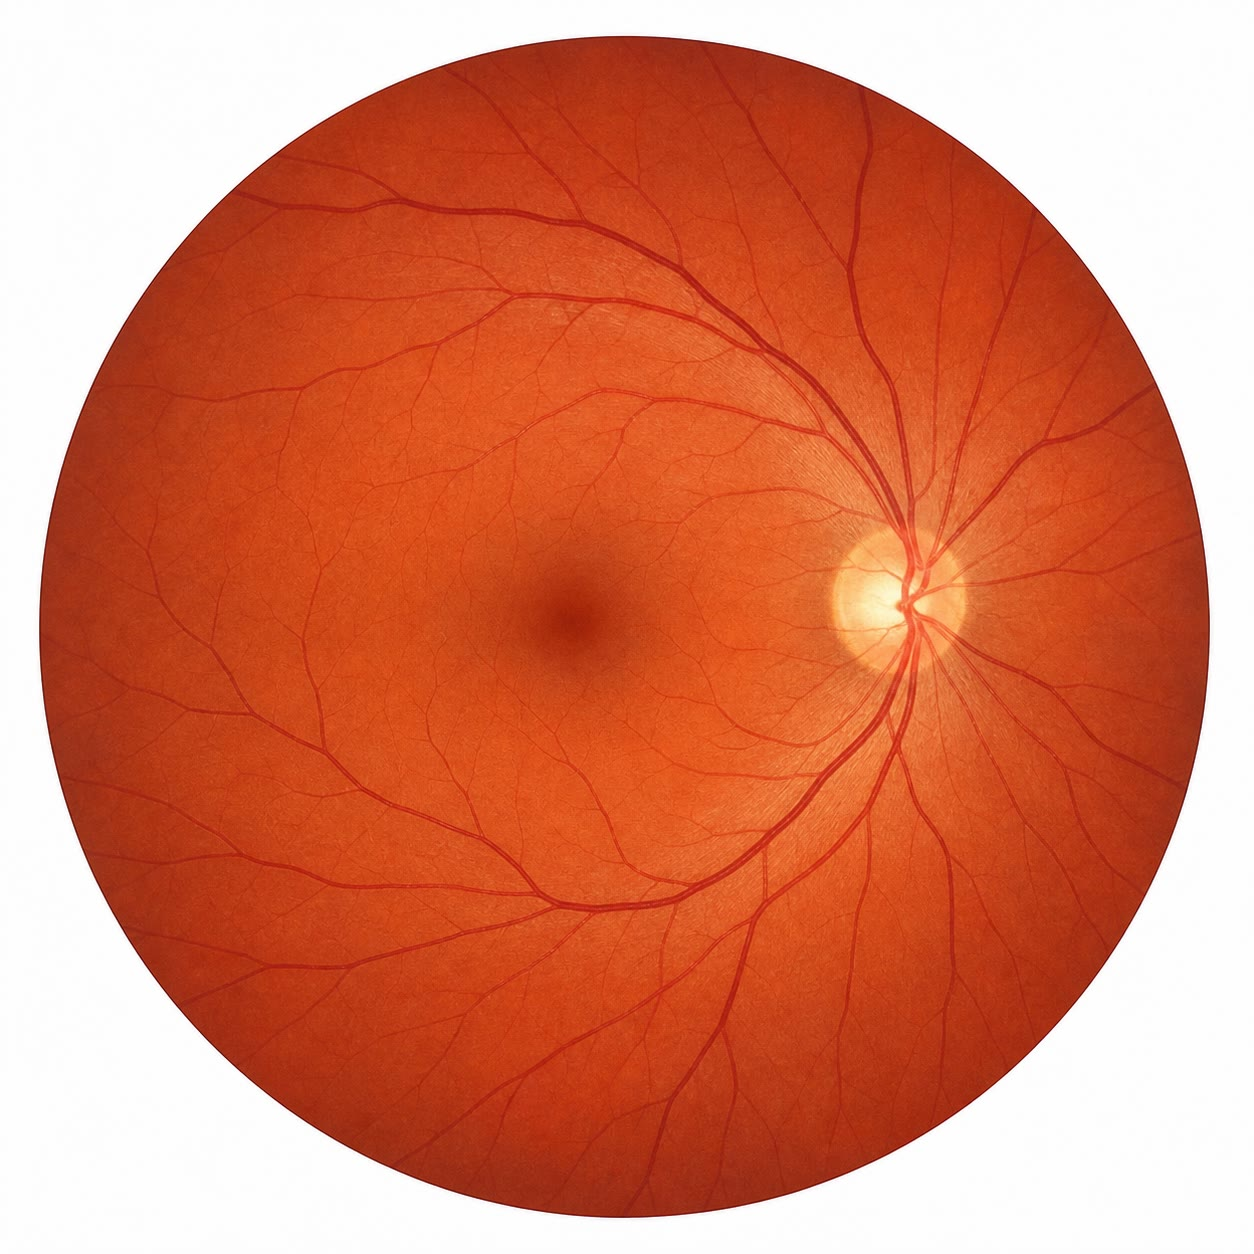
\includegraphics[width=0.42\linewidth]{images/book2/ai/g11-retina-fundus.jpg}

{\small La rétine vue à travers la pupille à l'ophtalmoscope~: le
disque pâle par où le nerf optique sort et les vaisseaux entrent (la
tache aveugle) et, plus sombre et sur le côté, la fovéa où les \omterm{def:g11:the-eye:photoreceptors}{cônes}
sont les plus denses.}
\end{omfigure}

\begin{example}[Les deux bizarreries expliquées]\label{ex:g11:the-eye:oddities}
L'étoile faible disparaît quand on la regarde en face parce que la
fovéa n'a que des \omterm{def:g11:the-eye:photoreceptors}{cônes}, qui exigent plus de lumière que l'étoile n'en
fournit~; regardée de côté, sa lumière tombe sur des \omterm{def:g11:the-eye:photoreceptors}{bâtonnets}, qui la
détectent. La veste est grise la nuit parce que les \omterm{def:g11:the-eye:photoreceptors}{bâtonnets} qui la
voient n'ont qu'un seul pigment~: ils peuvent rapporter combien de
lumière, non quelle longueur d'onde. La couleur est une comparaison
entre les trois types de \omterm{def:g11:the-eye:photoreceptors}{cônes}, et les \omterm{def:g11:the-eye:photoreceptors}{cônes} se taisent dans le noir.
\end{example}

\section{La couleur~: trois pigments}

\begin{proposition}[La vision des couleurs]\label{prop:g11:the-eye:colour}
Chaque type de cône contient l'une de trois \omterm{def:g11:the-eye:photoreceptors}{opsines}, dont les maxima
d'absorption se situent vers \qty{420}{nm} (\omterm{def:g11:the-eye:photoreceptors}{cônes} S, bleu),
\qty{530}{nm} (\omterm{def:g11:the-eye:photoreceptors}{cônes} M, vert) et \qty{560}{nm} (\omterm{def:g11:the-eye:photoreceptors}{cônes} L, rouge). Une
lumière donnée excite les trois types dans des proportions qui
dépendent de sa longueur d'onde~; le cerveau lit la couleur dans ces
proportions. Une personne privée d'un type de \omterm{def:g11:the-eye:photoreceptors}{cônes} confond les
couleurs que ce type distinguait~: sans \omterm{def:g11:the-eye:photoreceptors}{cônes} L ou M fonctionnels, le
rouge et le vert sont difficiles à distinguer --- c'est le
\emph{daltonisme rouge-vert}, qui touche environ 8~\% des hommes et
0.5~\% des femmes.
\end{proposition}
\admitted

\begin{omfigure}
\begin{tikzpicture}
\begin{axis}[
  width=0.9\linewidth, height=5.8cm,
  axis x line=bottom, axis y line=left,
  xmin=380, xmax=700, ymin=0, ymax=110,
  xlabel={longueur d'onde (nm)}, ylabel={absorption (\% du maximum)},
  xlabel style={font=\small, at={(axis description cs:0.5,-0.12)}, anchor=north},
  ylabel style={font=\small},
  tick label style={font=\small}, xtick={400,450,500,550,600,650,700}, ytick={0,50,100},
  legend style={at={(0.5,-0.3)}, anchor=north, legend columns=4, font=\small, draw=none},
]
\addplot[thick, omDef, smooth] coordinates {(380,40) (400,75) (420,100) (440,88) (460,55) (480,25) (500,8) (520,2) (540,0)};
\addplot[thick, gray, dashed, smooth] coordinates {(400,10) (430,35) (460,70) (480,90) (500,100) (520,90) (540,65) (560,38) (580,18) (600,7) (620,2) (640,0)};
\addplot[thick, omMeth, smooth] coordinates {(420,5) (450,20) (480,50) (510,85) (530,100) (550,90) (570,65) (590,38) (610,18) (630,7) (650,2) (670,0)};
\addplot[thick, omThm, smooth] coordinates {(440,5) (470,18) (500,40) (530,80) (560,100) (580,92) (600,70) (620,42) (640,20) (660,8) (680,3) (700,1)};
\legend{cônes S (bleu), bâtonnets, cônes M (vert), cônes L (rouge)}
\end{axis}
\end{tikzpicture}

{\small Absorption des quatre photopigments en fonction de la longueur
d'onde. Chacune est large et elles se recouvrent~; une lumière jaune de
\qty{580}{nm} excite fortement les \omterm{def:g11:the-eye:photoreceptors}{cônes} L, modérément les \omterm{def:g11:the-eye:photoreceptors}{cônes} M et
pas du tout les \omterm{def:g11:the-eye:photoreceptors}{cônes} S --- ce rapport est ce que «~jaune~» signifie
pour le cerveau.}
\end{omfigure}

\begin{example}[Lire les courbes]\label{ex:g11:the-eye:curves}
Lumière de \qty{500}{nm}~: \omterm{def:g11:the-eye:photoreceptors}{cônes} S à 8~\%, M à 75~\%, L à 40~\% ---
vue comme un bleu-vert. Lumière de \qty{620}{nm}~: S à 0, M à 10~\%, L
à 42~\% --- rouge. Une personne sans \omterm{def:g11:the-eye:photoreceptors}{cônes} L ne reçoit, pour les deux,
qu'une valeur S et une valeur M, et la seconde lumière donne S~0,
M~10~: à peine distinguable d'un vert faible. Les couleurs que le type
manquant aurait distinguées se confondent en une seule.
\end{example}

\section{Les gènes des opsines~: une famille et son histoire}

\begin{proposition}[Les gènes des opsines]\label{prop:g11:the-eye:genes}
Chaque \omterm{def:g11:the-eye:photoreceptors}{opsine} est codée par son propre \omterm{def:g10:universal-dna:gene}{gène}. Le \omterm{def:g10:universal-dna:gene}{gène} de l'\omterm{def:g11:the-eye:photoreceptors}{opsine} S est
porté par un \omterm{def:g11:cell-cycle-mitosis:chromosome}{chromosome} ordinaire~; les \omterm{def:g10:universal-dna:gene}{gènes} des \omterm{def:g11:the-eye:photoreceptors}{opsines} M et L sont
côte à côte sur le \omterm{def:g11:cell-cycle-mitosis:chromosome}{chromosome} X. Les \omterm{def:g10:chemistry-of-life:families}{protéines} L et M ne diffèrent que
par 15 de leurs 364 \omterm{def:g10:chemistry-of-life:families}{acides aminés} (96~\% d'identité), la \omterm{def:g11:gene-expression:protein}{protéine} S par
plus de la moitié de ses positions avec l'une ou l'autre. Étant sur
l'X, un \omterm{def:g10:universal-dna:gene}{allèle} M ou L non fonctionnel s'exprime chez tout homme qui le
porte et seulement chez les femmes qui en portent deux --- le schéma du
\cref{ch:g11:genes-and-disease}, et la raison pour laquelle le
daltonisme rouge-vert est seize fois plus fréquent chez les hommes.
\end{proposition}
\admitted

\begin{proposition}[Une famille de gènes née de duplications]\label{prop:g11:the-eye:family}
Les trois \omterm{def:g10:universal-dna:gene}{gènes} d'\omterm{def:g11:the-eye:photoreceptors}{opsines}, et celui du pigment des \omterm{def:g11:the-eye:photoreceptors}{bâtonnets}, sont des
versions d'un \omterm{def:g10:universal-dna:gene}{gène} ancestral copié par \emph{duplication} puis
divergeant par \omterm{def:g11:mutations:mutation}{mutation}. Leurs degrés de ressemblance datent les
copies~: les lignées S et L/M se sont séparées très tôt dans l'histoire
des \omterm{def:g10:common-ancestry:bodyplan}{vertébrés}, il y a quelque 500 millions d'années~; les \omterm{def:g10:universal-dna:gene}{gènes} L et M
sont nés d'une duplication il y a 30 à 40 millions d'années chez
l'ancêtre des primates de l'Ancien Monde, dont les descendants ---
singes, grands singes, humains --- ont trois types de \omterm{def:g11:the-eye:photoreceptors}{cônes} alors que
la plupart des autres mammifères en ont deux.
\end{proposition}
\begin{proof}[Faits expérimentaux]
La comparaison des séquences~: les \omterm{def:g10:universal-dna:gene}{gènes} L et M sont identiques à
96~\% et adjacents sur l'X --- la signature d'une duplication en
tandem récente~; chacun est identique à environ 43~\% au \omterm{def:g10:universal-dna:gene}{gène} S, et
tous trois à environ 40~\% au \omterm{def:g10:universal-dna:gene}{gène} de l'\omterm{def:g11:the-eye:photoreceptors}{opsine} des \omterm{def:g11:the-eye:photoreceptors}{bâtonnets}, copies
plus lointaines. Le chien, le bœuf et la plupart des mammifères
n'ont qu'un \omterm{def:g10:universal-dna:gene}{gène} d'\omterm{def:g11:the-eye:photoreceptors}{opsine} lié à l'X, à la place où les primates en ont
deux~; les singes du Nouveau Monde en ont un, avec plusieurs \omterm{def:g10:universal-dna:gene}{allèles},
et seules les femelles porteuses de deux \omterm{def:g10:universal-dna:gene}{allèles} différents voient
trois couleurs. Le nombre de \omterm{def:g10:universal-dna:gene}{gènes} correspond au nombre de types de
\omterm{def:g11:the-eye:photoreceptors}{cônes} dans chaque lignée, et l'arbre des \omterm{def:g10:universal-dna:gene}{gènes} correspond à l'arbre des
\omterm{def:g10:biodiversity-scales:species}{espèces}.
\end{proof}

\begin{omfigure}
\begin{tikzpicture}[font=\small, line cap=round]
  % gene tree: root -> (rod opsin) ; (S) ; (L/M split)
  \draw[thick] (0,2) -- (1.5,2);
  \draw[thick] (1.5,2) -- (1.5,3.4) -- (9,3.4);
  \draw[thick] (1.5,2) -- (1.5,0.6) -- (3.2,0.6);
  \draw[thick] (3.2,0.6) -- (3.2,1.8) -- (9,1.8);
  \draw[thick] (3.2,0.6) -- (3.2,-0.6) -- (7.6,-0.6);
  \draw[thick] (7.6,-0.6) -- (7.6,0.2) -- (9,0.2);
  \draw[thick] (7.6,-0.6) -- (7.6,-1.4) -- (9,-1.4);
  \fill[omThm] (1.5,2) circle (2.5pt); \fill[omThm] (3.2,0.6) circle (2.5pt); \fill[omThm] (7.6,-0.6) circle (2.5pt);
  \node[anchor=west] at (9.1,3.4) {rhodopsine (bâtonnets)};
  \node[anchor=west] at (9.1,1.8) {opsine S (cônes bleus)};
  \node[anchor=west] at (9.1,0.2) {opsine M (cônes verts)};
  \node[anchor=west] at (9.1,-1.4) {opsine L (cônes rouges)};
  \node[anchor=south, font=\scriptsize, omThm] at (1.5,3.5) {duplication ancienne};
  \node[anchor=north, font=\scriptsize, omThm, align=center] at (3.2,-0.75) {duplication\\ $\sim$500 millions d'années};
  \node[anchor=north, font=\scriptsize, omThm, align=center] at (7.6,-1.55) {duplication\\ $\sim$35 millions d'années};
  \node[anchor=east] at (-0.1,2) {gène ancestral};
  \draw[->, gray] (0,-2.3) -- (9,-2.3) node[midway, below, font=\scriptsize] {temps};
\end{tikzpicture}

{\small La famille des \omterm{def:g10:universal-dna:gene}{gènes} d'\omterm{def:g11:the-eye:photoreceptors}{opsines}. Chaque point rouge est une
duplication~: un \omterm{def:g10:universal-dna:gene}{gène} en est devenu deux, et les copies ont ensuite
divergé par \omterm{def:g11:mutations:mutation}{mutation}. La plus récente, L/M, ne se rencontre que chez
les primates de l'Ancien Monde et leur a donné un troisième cône.}
\end{omfigure}

\begin{example}[Ce qu'a changé une duplication]\label{ex:g11:the-eye:duplication}
Un singe à deux types de \omterm{def:g11:the-eye:photoreceptors}{cônes} voit la forêt en deux dimensions de
couleur, et un fruit mûr se détache mal du feuillage. Après la
duplication L/M, une copie a pu muter vers les grandes longueurs d'onde
pendant que l'autre gardait l'original --- un troisième cône, et le
rouge mûr sur fond vert. La \omterm{def:g11:mutations:mutation}{mutation} qui casse plus tard l'une des
copies chez 8~\% des hommes ne fait que ramener l'\omterm{def:g11:the-eye:parts}{œil} à l'état
ancestral à deux \omterm{def:g11:the-eye:photoreceptors}{cônes}.
\end{example}

\begin{method}[Raisonner sur un cas de vision des couleurs]\label{met:g11:the-eye:case}
\begin{enumerate}
  \item Quel type de \omterm{def:g11:the-eye:photoreceptors}{cônes} manque ou est modifié~? Le lire dans les
        couleurs confondues (rouge-vert~: L ou M~; bleu-jaune, rare~:
        S).
  \item Quel \omterm{def:g10:universal-dna:gene}{gène}, et sur quel \omterm{def:g11:cell-cycle-mitosis:chromosome}{chromosome}~? L et M sur l'X, S
        ailleurs.
  \item Appliquer la transmission~: récessive liée à l'X pour le
        rouge-vert --- les fils de mères porteuses atteints une fois
        sur deux, les filles de pères atteints toutes porteuses.
  \item Rapporter à la famille de \omterm{def:g10:universal-dna:gene}{gènes}~: une copie perdue, ou une
        copie L et une copie M rendues trop semblables par un échange
        entre les \omterm{def:g10:universal-dna:gene}{gènes} voisins.
\end{enumerate}
\end{method}

\begin{remark}[De l'œil au cerveau]\label{rem:g11:the-eye:tobrain}
La rétine ne voit pas~; elle convertit et commence à trier. Le million
de fibres du nerf optique porte une description codée --- contrastes,
contours, rapports des réponses des \omterm{def:g11:the-eye:photoreceptors}{cônes} --- jusqu'au cerveau, où le
chapitre suivant la reprend. Ce que nous appelons voir se passe là,
bâti sur les signaux des \omterm{def:g10:cells-common-unit:cell}{cellules} décrites ici et sur rien d'autre~:
une personne dont les rétines fonctionnent mais dont le cerveau visuel
est lésé est aveugle, et une personne dont le cerveau visuel fonctionne
mais dont les \omterm{def:g11:the-eye:photoreceptors}{photorécepteurs} sont morts l'est aussi.
\end{remark}

\section{Exercices}

\begin{exercise}[$\star$]\label{exo:g11:the-eye:1}
Énumérer, dans l'ordre, les structures que la lumière traverse de
l'extérieur jusqu'aux \omterm{def:g11:the-eye:photoreceptors}{photorécepteurs}.
\end{exercise}

\begin{exercise}[$\star$]\label{exo:g11:the-eye:2}
Comparer \omterm{def:g11:the-eye:photoreceptors}{bâtonnets} et \omterm{def:g11:the-eye:photoreceptors}{cônes}~: nombre, sensibilité, pigments, type de
vision.
\end{exercise}

\begin{exercise}[$\star$]\label{exo:g11:the-eye:3}
Qu'est-ce que la fovéa~? Et la tache aveugle~?
\end{exercise}

\begin{exercise}[$\star$]\label{exo:g11:the-eye:4}
D'après la figure des absorptions, quels pigments absorbent une lumière
de \qty{450}{nm}, et avec quelle intensité~?
\end{exercise}

\begin{exercise}[$\star$]\label{exo:g11:the-eye:5}
Sur quel \omterm{def:g11:cell-cycle-mitosis:chromosome}{chromosome} se trouvent les \omterm{def:g10:universal-dna:gene}{gènes} des \omterm{def:g11:the-eye:photoreceptors}{opsines} L et M, et
qu'est-ce qui en découle pour la transmission du daltonisme
rouge-vert~?
\end{exercise}

\begin{exercise}[$\star\star$]\label{exo:g11:the-eye:6}
Expliquer pourquoi nous ne voyons pas les couleurs la nuit, et pourquoi
une étoile faible se voit mieux de côté.
\end{exercise}

\begin{exercise}[$\star\star$]\label{exo:g11:the-eye:7}
Deux lumières excitent les \omterm{def:g11:the-eye:photoreceptors}{cônes} ainsi~: lumière 1, S 0, M 60, L 100~;
lumière 2, S 0, M 30, L 50. Sont-elles de la même couleur~? De la même
luminosité~? Expliquer.
\end{exercise}

\begin{exercise}[$\star\star$]\label{exo:g11:the-eye:8}
Un homme daltonien épouse une femme sans parent daltonien. Donner la
vision des couleurs de leurs fils, de leurs filles et des fils de leurs
filles.
\end{exercise}

\begin{exercise}[$\star\star$]\label{exo:g11:the-eye:9}
Pourquoi le daltonisme rouge-vert est-il seize fois plus fréquent chez
les hommes que chez les femmes~? Calculer la fréquence attendue chez
les femmes à partir des 8~\% chez les hommes.
\end{exercise}

\begin{exercise}[$\star\star$]\label{exo:g11:the-eye:10}
Les \omterm{def:g10:universal-dna:gene}{gènes} L et M sont identiques à 96~\%, chacun à 43~\% au \omterm{def:g10:universal-dna:gene}{gène} S.
Expliquer comment ces deux nombres datent les duplications l'une par
rapport à l'autre.
\end{exercise}

\begin{exercise}[$\star\star$]\label{exo:g11:the-eye:11}
La plupart des mammifères ont deux types de \omterm{def:g11:the-eye:photoreceptors}{cônes}, les primates de
l'Ancien Monde trois. Expliquer la différence par une duplication, et
dire pourquoi elle a pu être conservée.
\end{exercise}

\begin{exercise}[$\star\star\star$]\label{exo:g11:the-eye:12}
Une personne est privée des \omterm{def:g11:the-eye:photoreceptors}{cônes} S. Quelles couleurs confond-elle~?
Expliquer pourquoi cet état est rare et également fréquent dans les
deux sexes.
\end{exercise}

\begin{exercise}[$\star\star\star$]\label{exo:g11:the-eye:13}
Les \omterm{def:g11:the-eye:photoreceptors}{cônes} de la fovéa sont espacés de \qty{2.5}{\micro m} et la
distance focale de l'\omterm{def:g11:the-eye:parts}{œil} vaut environ \qty{17}{mm}. Calculer le plus
petit angle sous lequel deux points peuvent être vus tout en tombant
sur des \omterm{def:g11:the-eye:photoreceptors}{cônes} distincts, et la taille du plus petit détail résoluble à
\qty{10}{m}. (Utiliser l'approximation des petits angles~: angle en
radians $=$ taille $/$ distance.)
\end{exercise}

\begin{exercise}[$\star\star\star$]\label{exo:g11:the-eye:14}
Chez les singes du Nouveau Monde, l'unique \omterm{def:g10:universal-dna:gene}{gène} d'\omterm{def:g11:the-eye:photoreceptors}{opsine} lié à l'X a
plusieurs \omterm{def:g10:universal-dna:gene}{allèles} de longueurs d'onde maximales différentes. Expliquer
pourquoi seules certaines femelles de ces \omterm{def:g10:biodiversity-scales:species}{espèces} voient trois
couleurs, et aucun mâle.
\end{exercise}

\begin{exercise}[$\star\star\star$]\label{exo:g11:the-eye:15}
Une maladie détruit les \omterm{def:g11:the-eye:photoreceptors}{photorécepteurs} mais épargne le reste de la
rétine. Expliquer pourquoi un implant qui stimule électriquement les
\omterm{def:g10:cells-common-unit:cell}{cellules} ganglionnaires peut restaurer une vision partielle, et ce qui
en limite la qualité.
\end{exercise}

\section{Problème~: trois pigments et une duplication}

\begin{problem}[{Problème du week-end --- la vision des couleurs
démontée~: les réponses des cônes à un spectre, une famille touchée par
le daltonisme, les gènes d'opsines comparés, et la finesse qu'une fovéa
peut atteindre}]
\label{pb:g11:the-eye:1}
On utilisera la figure des absorptions. Un test présente des lumières
de \qty{470}{nm}, \qty{530}{nm}, \qty{590}{nm} et \qty{650}{nm}.

\medskip
\noindent\textbf{Partie I --- Les \omterm{def:g11:the-eye:photoreceptors}{cônes} répondent.}
\begin{enumerate}
  \item Pour chaque lumière, lire la réponse approchée des \omterm{def:g11:the-eye:photoreceptors}{cônes} S, M
        et L.
  \item Quelle lumière excite les trois types~? Laquelle n'en excite
        qu'un~?
  \item Une personne privée de \omterm{def:g11:the-eye:photoreceptors}{cônes} L ne reçoit que les valeurs S et
        M. Lesquelles des quatre lumières lui deviennent difficiles à
        distinguer~? Justifier par les nombres.
  \item Une personne privée de \omterm{def:g11:the-eye:photoreceptors}{cônes} M~: quelle paire confond-elle~?
  \item Expliquer pourquoi aucune des deux n'est «~aveugle au rouge~»
        et pourquoi toutes deux distinguent mal le rouge du vert.
\end{enumerate}

\medskip
\noindent\textbf{Partie II --- Une famille.}
Nora voit les couleurs normalement~; son père est daltonien
rouge-vert. Elle épouse Sam, qui voit normalement.
\begin{enumerate}[resume]
  \item Donner le \omterm{def:g11:enzymes-and-phenotype:phenotype}{génotype} de Nora pour le \omterm{def:g10:universal-dna:gene}{gène} d'\omterm{def:g11:the-eye:photoreceptors}{opsine} lié à l'X, et
        le justifier.
  \item Donner les \omterm{def:g11:enzymes-and-phenotype:phenotype}{génotypes} et la vision des couleurs de leurs fils et
        filles possibles, avec les probabilités.
  \item Leur fille Inès, dont la vision des couleurs est normale,
        épouse un homme daltonien. Calculer la probabilité qu'Inès soit
        porteuse, puis la probabilité qu'une de leurs filles soit
        daltonienne.
  \item Expliquer pourquoi une fille daltonienne a toujours un père
        daltonien.
  \item La mère du père de Nora voyait les couleurs normalement.
        Était-elle nécessairement porteuse~? Expliquer.
\end{enumerate}

\medskip
\noindent\textbf{Partie III --- Les \omterm{def:g10:universal-dna:gene}{gènes}.}
Identités entre les séquences protéiques des \omterm{def:g11:the-eye:photoreceptors}{opsines}~: L--M 96~\%,
L--S 43~\%, M--S 43~\%, S--rhodopsine 41~\%.
\begin{enumerate}[resume]
  \item Dessiner, ou décrire, l'arbre des quatre \omterm{def:g10:universal-dna:gene}{gènes} qu'impliquent
        ces nombres.
  \item Si les différences s'accumulent à vitesse constante et si la
        duplication L/M date de 35 millions d'années, estimer l'âge de
        la séparation entre S et la lignée L/M.
  \item Les \omterm{def:g10:universal-dna:gene}{gènes} L et M sont côte à côte sur l'X. Expliquer comment un
        échange inégal entre eux au cours de la méiose peut produire un
        X ne portant qu'un des deux, et quelle vision des couleurs en
        résulte.
  \item De tels échanges sont la cause la plus fréquente du daltonisme
        rouge-vert. Pourquoi deux \omterm{def:g10:universal-dna:gene}{gènes} voisins et presque identiques
        y sont-ils particulièrement exposés~?
  \item La duplication L/M se rencontre chez tous les primates de
        l'Ancien Monde et chez aucun autre mammifère. Que cela dit-il
        du moment où elle est survenue et de qui l'a subie~?
\end{enumerate}

\medskip
\noindent\textbf{Partie IV --- La finesse de la fovéa.}
Les \omterm{def:g11:the-eye:photoreceptors}{cônes} de la fovéa sont espacés de \qty{2.5}{\micro m}~; la distance
focale de l'\omterm{def:g11:the-eye:parts}{œil} vaut \qty{17}{mm}. Utiliser angle (radians) $=$ taille
$/$ distance.
\begin{enumerate}[resume]
  \item Calculer l'angle sous-tendu par deux \omterm{def:g11:the-eye:photoreceptors}{cônes} voisins, en radians
        puis en minutes d'arc ($1' = \num{2.9e-4}$ rad).
  \item Quel est le plus petit détail de lettre résoluble à
        \qty{6}{m}~? Comparer aux traits des lettres d'une échelle
        d'acuité visuelle, environ \qty{1.7}{mm} à cette distance pour
        une vision «~normale~».
  \item Loin de la fovéa, 100 \omterm{def:g11:the-eye:photoreceptors}{bâtonnets} partagent une \omterm{def:g10:cells-common-unit:cell}{cellule}
        ganglionnaire. Estimer l'angle résoluble là-bas, et expliquer
        ce qu'on gagne en échange.
  \item Les \omterm{def:g11:the-eye:photoreceptors}{cônes} fovéaux d'un aigle sont deux fois plus denses et son
        \omterm{def:g11:the-eye:parts}{œil} un peu plus grand. De quel facteur sa \omterm{def:g10:cells-common-unit:magnification}{résolution} est-elle
        plus fine~?
  \item Énoncer le résultat~: les trois types de \omterm{def:g11:the-eye:photoreceptors}{cônes} et la lumière à
        laquelle chacun est aveugle, l'unique événement génétique qui a
        donné le troisième aux primates, et l'angle que la fovéa résout.
\end{enumerate}
\end{problem}
